\documentclass{beamer}
\usetheme{Madrid}
\colorlet{beamer@blendedblue}{green!40!black}
\setbeamertemplate{caption}[numbered]
\usepackage{amssymb, amsmath, amsthm}
\usepackage{physics, siunitx}
\usepackage{float, subcaption, graphicx, wrapfig2}
\usepackage{hyperref}

\title{Introduction to Compact Torus}
\author{Hunt Feng\inst{1}}
\institute[Usask]
{
	\inst{1}%
	Department of Physics and Engineering Physics\\
	University of Saskatchewan
}
\date{\today}

%%%%%%%%%%%%%%%%%%%%
% section page 
%%%%%%%%%%%%%%%%%%%%
\AtBeginSection[]
{
	\begin{frame}{Outline of Presentation}
		\tableofcontents[currentsection]
	\end{frame}
}

\begin{document}
%%%%%%%%%%%%%%%%%%%%
% title and TOC
%%%%%%%%%%%%%%%%%%%%
\maketitle
\begin{frame}{Outline of Presentation}
	\tableofcontents
\end{frame}

%%%%%%%%%%%%%%%%%%%%
% contents 
%%%%%%%%%%%%%%%%%%%%
\section{Compact Torus (CT)}
\begin{frame} {Starting From Nuclear Fusion}
    In order to make fusion energy a viable economic alternative, significant improvements in concept design need to occur.
    \begin{itemize}
        \item We want the device to be \textbf{Simply connected}. Meaning that there is no material linking the center of the device, making the first wall either a sphere or a cylinder.
        \item By removing the center material of the device, the cost decreases and the engineering becomes simple.
        \item Compact Torus suits this purpose very well.
    \end{itemize}
\end{frame}

\begin{frame} {Well Studied CTs}
    \begin{itemize}
        \item Compact torus is a toroidal magnetic configuration with a simply-connected geometry that are self-stable.
    \end{itemize}

    The following configurations fall into the category of compact torus:
    \begin{itemize}
        \item Spheromak.
        \item Field-reversed configuration (FRC).
        \item Particle ring. (Not in active research today.)
    \end{itemize}
\end{frame}

\begin{frame} {Spheromak}
    \begin{itemize}
        \item Spheromak is a toroidal confinement with toroidal and poloidal fields.
        \item Toroidal field is completely generated by plasma currents.
        \item The current is toroidal at the core and poloidal at the surface.
        \item The current is parallel to $\mathbf{B}$ in spheromak, $\grad p = \mathbf{j\times B}=0$.
        \item Ideally it is always MHD stable. In reality, spheromak has finite pressure and due to different decay rates of toroidal and poloidal fields, current driven kink modes will be developed.
    \end{itemize}

    \begin{figure}
        \centering
        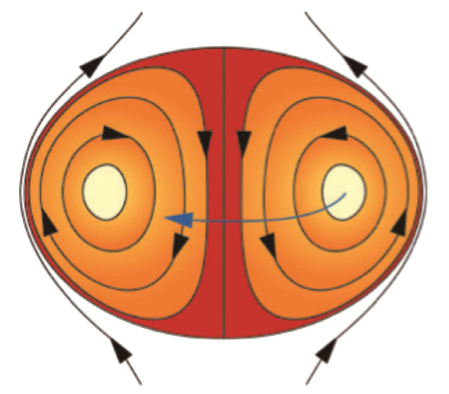
\includegraphics[width=0.3\textwidth]{figures/sphromak.png}
        \caption{Spheromak configuration. \cite{gao_2016_compact} The arrow lines are magnetic field lines.}
        \label{fig:spheromak}
    \end{figure}

    \tiny \cite{gao_2016_compact} Z.Gao. \textit{Compact magnetic confinement fusion: Spherical torus and compact torus.}
\end{frame}

\begin{frame} {Spheromak Issues \cite{gao_2016_compact}}
    \begin{itemize}
        \item Due to absence of toroidal field coils, it is difficult to generate large toroidal fields in spheromak.
        \item Due to absence of ohmic coils, it is difficult to obtain long pulse discharges.
        \item The above issues indicates: it is hard to achieve good confinement simultaneously with an efficient current drive. The drive of plasma current will break the magnetic surface and induce high-level heat losses.
    \end{itemize}
\end{frame}

\begin{frame} {Spheromak Successes \cite{woodruff_2008_technical}}
    \begin{itemize}
        \item Tokamak-like transport measured in the SSPX experiment by suppressing fluctuations.
        \item Multi-pulsed build-up of magnetic energy in a spheromak demonstrated in SSPX.
        \item SSX merged spheromaks and detailed magnetic reconnection and generation of energetic plasma flows, FRC formation by merging.
        \item TS-3/4 shows means for forming various toroidal configurations by merging.
    \end{itemize}
\end{frame}

\begin{frame} {Field Reversed Configuration (FRC)}
    \begin{itemize}
        \item FRC is a toroidal confinement with poloidal field only.
        \item Bulk currents of FRC are diamagnetic, leading to a high beta $\sim$ 1.
        \item FRC equilibrium cannot be described by Grad-Shafranov equation. Two-fluid or kinetic theory is needed.
        \item FRC's magnetic topology indicates that it is unstable to most ideal MHD modes, but robust stability can be obtained in experiments.
    \end{itemize}

    \begin{figure}
        \centering
        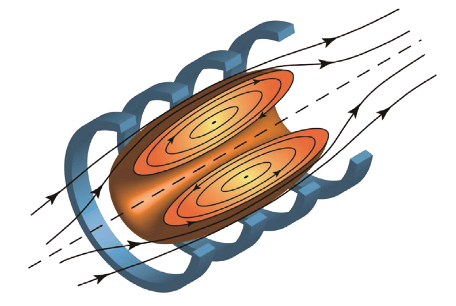
\includegraphics[width=0.3\textwidth]{figures/frc.png}
        \caption{Field reversed configuration. \cite{gao_2016_compact} Arrow lines are magnetic field lines.}
        \label{fig:frc}
    \end{figure}

    \tiny \cite{gao_2016_compact} Z.Gao. \textit{Compact magnetic confinement fusion: Spherical torus and compact torus.}
\end{frame}

\begin{frame} {FRC Issues \cite{gao_2016_compact}}
    \begin{itemize}
        \item It is believed that Finite Larmor radius (FLR) effect contributes to the stability, but this effect is not effective in large-size FRC.
        \item Sheared flows and large orbit of energetic ions may improve stability but theoretical explanations and experimental evidences are not well convincing.
        \item FRC provides a big challenge in equilibrium and stability of plasmas at the extreme.
    \end{itemize}
\end{frame}

\begin{frame} {FRC Successes \cite{woodruff_2008_technical}}
    \begin{itemize}
        \item Formation and Sustainment of long-lived FRCs in the TCS device (10 ms).
        \item Production of low-density FRCs with enhanced confinement in Osaka FIX experiment.
        \item Production of high density FRCs in the FRX-L device. FRCs have been formed with an equilibrium density $n_e (\sim 1-2) 10^{16}$\unit{\cm^{-3}}, $T_e < T_i \sim 250$\unit{eV}, and excluded flux $2-3$\unit{\milli\weber}.
        \item Formation, acceleration to $M > 1$, and collisions of FRCs in the IPA device.
    \end{itemize}
\end{frame}

\begin{frame} {Comparison Among Configurations}
    \begin{itemize}
        \item CT can be used in fusion technology.
    \end{itemize}
    \begin{figure}
        \centering
        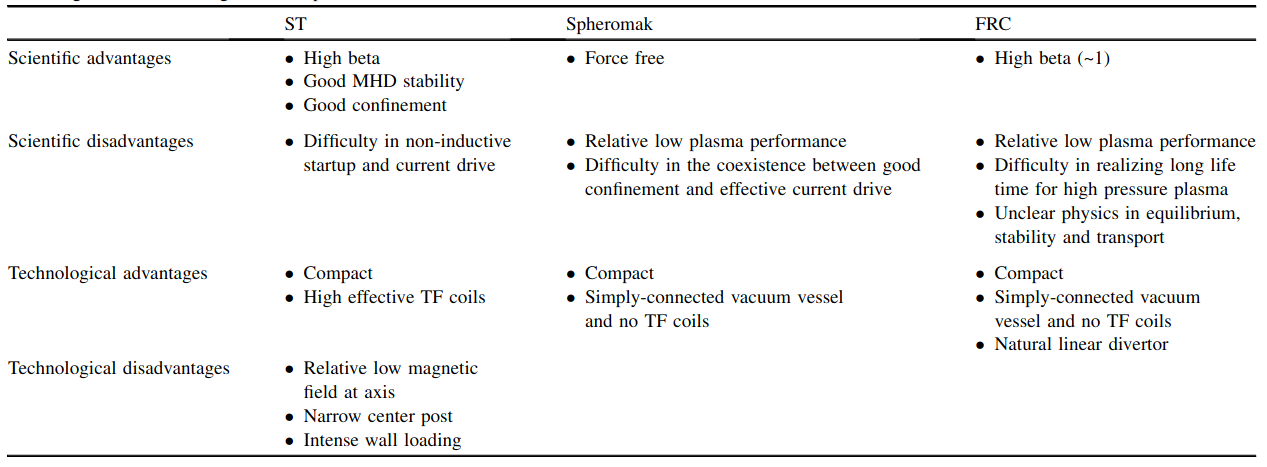
\includegraphics[width=\textwidth]{figures/comparisons.png}
        \caption{Advantages and disadvantages of Spherical Tokamak (ST), spheromak and FRC for fusion. \cite{gao_2016_compact}}
        \label{fig:comparisons}
    \end{figure}

    \tiny \cite{gao_2016_compact} Z.Gao. \textit{Compact magnetic confinement fusion: Spherical torus and compact torus.}
\end{frame}

\begin{frame} {Plasma Performance Achievements}
    \begin{figure}
        \centering
        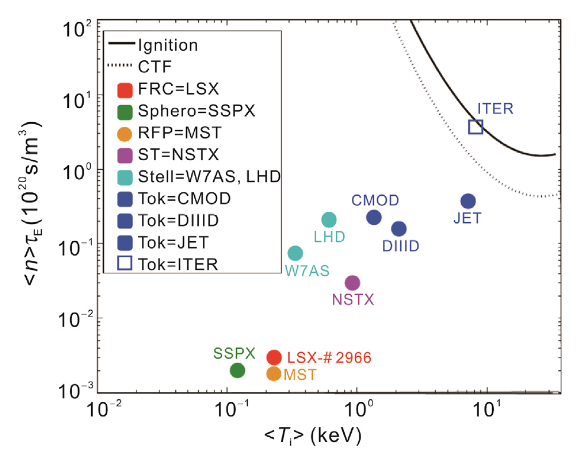
\includegraphics[width=0.7\textwidth]{figures/plasma-performance.png}
        \caption{Plasma performance achievements of various concepts. \cite{gao_2016_compact}}
        \label{fig:plasma-performance}
    \end{figure}

    \tiny \cite{gao_2016_compact} Z.Gao. \textit{Compact magnetic confinement fusion: Spherical torus and compact torus.}
\end{frame}
\section{Magnetized Target Fusion (MTF)}
\begin{frame} {Magnetized Target Fusion (MTF)}
    \begin{itemize}
        \item To obtain high pressure in magnetic confinement fusion (MCF): need to improve confinement time and/or enlarge the machine size.
        \item To obtain high pressure in inertial confinement fusion (ICF): compress small size plasma to ultra-high density but stability degrades the compression efficiency.
        \item MCF is a combination of MCF and ICF: compressing a magnetically confined plasma.
    \end{itemize}
\end{frame}

\begin{frame} {MTF Concept}
    \begin{figure}
        \centering
        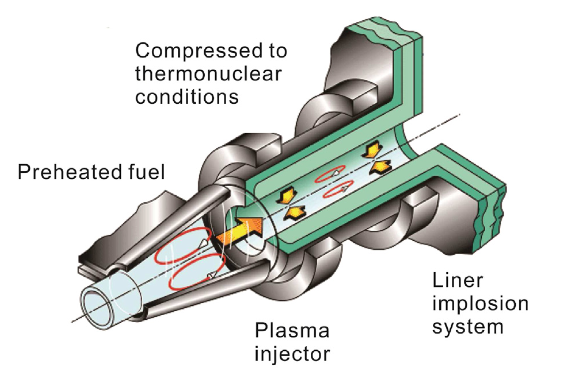
\includegraphics[width=0.6\textwidth]{figures/mtf-concept.png}
        \caption{Schematic of MTF concept. \cite{gao_2016_compact}}
        \label{fig:mtf-concept}
    \end{figure}

    \tiny \cite{gao_2016_compact} Z.Gao. \textit{Compact magnetic confinement fusion: Spherical torus and compact torus.}
\end{frame}

\begin{frame}[t] {MTF at General Fusion}
    \begin{wrapfigure}{l}{0.4\textwidth}
        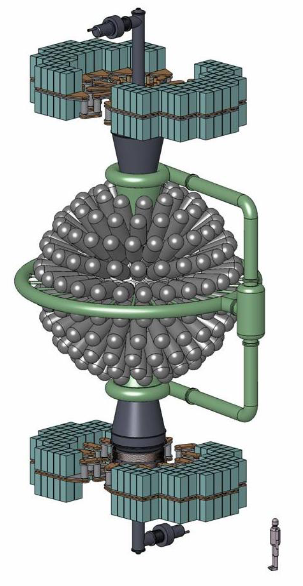
\includegraphics[height=0.6\textheight]{figures/mtf-at-general-fusion.png}
        \caption{General Fusion's Acoustic Magnetized Target Fusion Reactor Concept. \cite{delage_2012_progress}}
        \label{fig:mtf-at-general-fusion}
    \end{wrapfigure}

    The early MTF concept in General Fusion involves the compact torus.
    \begin{itemize}
        \item The deterium-tritium fuel is supplied as a pair of CTs (spheromaks).
        \item CT accelerators are at the poles.
        \item Injected CTs travel to the center and merge to form a stationary compressible plasma target.
        \item The target is compressed by acoustic pressure.
        \item The acoustic pulse is generated mechanically by hundreds of pneumatically-driven pistons.
    \end{itemize}

    \tiny \cite{delage_2012_progress}  M. Delage, A. Froese, D. Blondal, and D. Richardson. \textit{Progress towards acoustic magnetized target fusion: An overview of the r\&d program at general fusion.}
\end{frame}
\section{Compact Torus Injector}
\begin{frame} {Central Fuelling of Tokamak}
    Central fuelling can:
    \begin{itemize}
        \item control plasma density and pressure profiles.
        \item make plasma to achieve high fuel burn-up rate and low tritium recycling.
        \item improve tokamak confinement.
    \end{itemize}

    However, conventional fuelling technologies (peripheral gas admission, and frozen pellet injection) have drawbacks:
    \begin{itemize}
        \item relatively low pellet speed prevents the direct fuel deposition beyond the separatrix in reactor-grade tokamak such as ITER.
        \item Energetic neutral beam injection is economically inefficient.
    \end{itemize}
\end{frame}

\begin{frame} {Compact Torus Injection}
    New injection technology, CT injection has some benefits:
    \begin{itemize}
        \item CT can be accelerated to hundreds of kilometers per second.
        \item Tangential CT injection may transfer CT momentum to tokamak plasma to induce and sustain toroidal rotation, good for stabilizing the locked mode and resistive wall mode.
        \item It is observed that tangential CT injection into STOR-M tokamak induces H-mode discharges.
    \end{itemize}
\end{frame}

\begin{frame} {Tangential Compact Torus Injection Setup}
    \begin{figure}
        \centering
        \begin{subfigure}{0.6\textwidth}
            \centering
            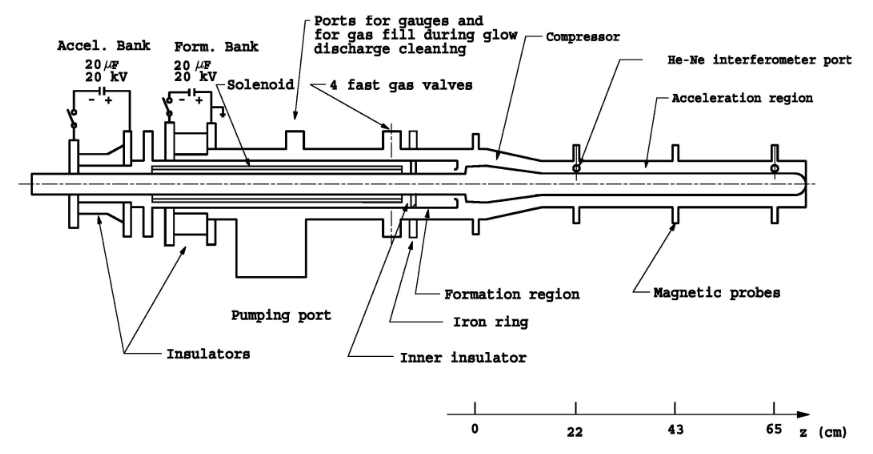
\includegraphics[width=\textwidth]{figures/uscti.png}
            \caption{Schematic diagram of USCTI. \cite{xiao_2004_improved}}
            \label{fig:uscti}
        \end{subfigure}%
        \begin{subfigure}{0.4\textwidth}
            \centering
            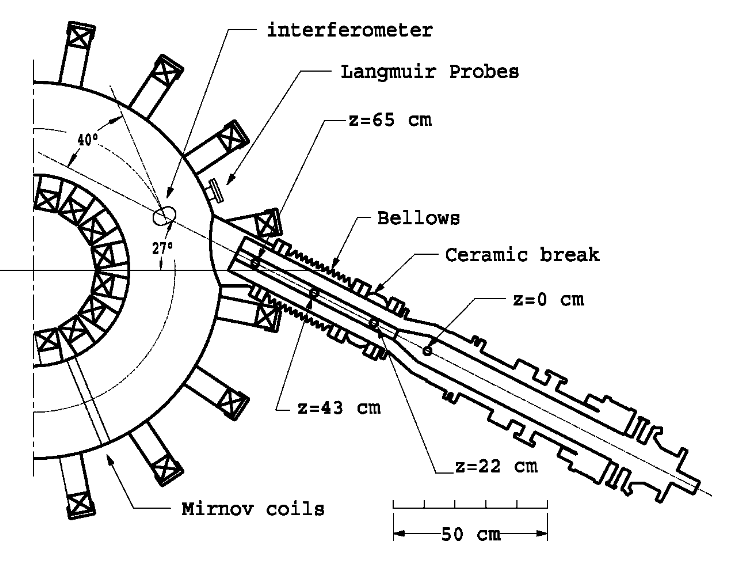
\includegraphics[width=\textwidth]{figures/tangential-cti-setup.png}
            \caption{Arrangement of CT injection experiments on the STOR-M tokamak. \cite{xiao_2004_improved}}
            \label{fig:tangential-cti-setup}
        \end{subfigure}
    \end{figure}

    \tiny \cite{xiao_2004_improved} C.Xiao, A. Hirose, and S.Sen. \textit{Improved confinement induced by tangential injection of compact torus into the saskatchewan torus-modified (stor-m) tokamak.}
\end{frame}

%%%%%%%%%%%%%%%%%%%%
% references
%%%%%%%%%%%%%%%%%%%%
\newpage
\begin{frame}[allowframebreaks]
	\bibliographystyle{abbrv}
	\bibliography{../references}
	\nocite{*}
\end{frame}

\end{document}